\documentclass[conference,compsoc]{IEEEtran}

\ifCLASSOPTIONcompsoc
  % IEEE Computer Society needs nocompress option
  % requires cite.sty v4.0 or later (November 2003)
  \usepackage[nocompress]{cite}
  \usepackage[utf8]{inputenc}
\else
  % normal IEEE
  \usepackage{cite}
\fi
% cite.sty was written by Donald Arseneau
% V1.6 and later of IEEEtran pre-defines the format of the cite.sty package
% \cite{} output to follow that of the IEEE. Loading the cite package will
% result in citation numbers being automatically sorted and properly
% "compressed/ranged". e.g., [1], [9], [2], [7], [5], [6] without using
% cite.sty will become [1], [2], [5]--[7], [9] using cite.sty. cite.sty's
% \cite will automatically add leading space, if needed. Use cite.sty's
% noadjust option (cite.sty V3.8 and later) if you want to turn this off
% such as if a citation ever needs to be enclosed in parenthesis.
% cite.sty is already installed on most LaTeX systems. Be sure and use
% version 5.0 (2009-03-20) and later if using hyperref.sty.
% The latest version can be obtained at:
% http://www.ctan.org/pkg/cite
% The documentation is contained in the cite.sty file itself.
%
% Note that some packages require special options to format as the Computer
% Society requires. In particular, Computer Society  papers do not use
% compressed citation ranges as is done in typical IEEE papers
% (e.g., [1]-[4]). Instead, they list every citation separately in order
% (e.g., [1], [2], [3], [4]). To get the latter we need to load the cite
% package with the nocompress option which is supported by cite.sty v4.0
% and later.

% *** GRAPHICS RELATED PACKAGES ***
%
\ifCLASSINFOpdf
  % \usepackage[pdftex]{graphicx}
  % declare the path(s) where your graphic files are
  % \graphicspath{{../pdf/}{../jpeg/}}
  % and their extensions so you won't have to specify these with
  % every instance of \includegraphics
  % \DeclareGraphicsExtensions{.pdf,.jpeg,.png}
\else
  % or other class option (dvipsone, dvipdf, if not using dvips). graphicx
  % will default to the driver specified in the system graphics.cfg if no
  % driver is specified.
  % \usepackage[dvips]{graphicx}
  % declare the path(s) where your graphic files are
  % \graphicspath{{../eps/}}
  % and their extensions so you won't have to specify these with
  % every instance of \includegraphics
  % \DeclareGraphicsExtensions{.eps}
\fi

% correct bad hyphenation here
\hyphenation{op-tical net-works semi-conduc-tor}


\usepackage{enumitem}
\usepackage{graphicx}
\usepackage{scrextend}
\usepackage{pgfplots}
\usepackage[portuguese]{babel}

\usepgfplotslibrary{groupplots}
\pgfplotsset{compat=1.12}
\usetikzlibrary{patterns}
\usepackage{ntheorem}


\graphicspath{ {./images/} }

\theoremseparator{:}
\newtheorem{hyp}{Hipótese}
\renewcommand\figurename{Figura}

\begin{document}
%
% paper title
% Titles are generally capitalized except for words such as a, an, and, as,
% at, but, by, for, in, nor, of, on, or, the, to and up, which are usually
% not capitalized unless they are the first or last word of the title.
% Linebreaks \\ can be used within to get better formatting as desired.
% Do not put math or special symbols in the title.
\title{Um Estudo de Performance entre Servidor Web PHP e Node.js}
\label{title}

% author names and affiliations
% use a multiple column layout for up to three different
% affiliations
\author{\IEEEauthorblockN{Luana Martins dos Santos}
\IEEEauthorblockA{Universidade Federal de Pernambuco\\
Centro de Informática\\
Recife, Pernambuco\\
Email: lms7@cin.ufpe.br}}

% make the title area
\maketitle

\label{abstract}
\begin{abstract}
Este artigo apresenta um estudo comparativo entre duas tecnologias para desenvolvimento \textit{server-side} de serviços \textit{web}. Entre elas, PHP, que é um framework bastante utilizado na indústria, enquanto que Node.js é mais recente. As tecnologias analisadas foram obtidas através de projetos do Github que realizam, entre outras funcionalidades, \textit{download} de arquivos. Para analisar os servidores, foram feitas simulações de \textit{download} de arquivos de tamanhos diferentes, considerando três variáveis, tempo de conexão, tempo de transferência e o total total da requisição. Obtidas essas métricas, foram feitas considerações sobre as variáveis necessárias para identificar qual dessas tecnologias, (...)

\end{abstract}

\IEEEpeerreviewmaketitle

\section{Introdução}
\label{introducao}
Com o avanço da internet, a utilização de \textit{webservices} tornou-se uma forma muito interessante de prover serviços de maneira simples. Os usuários precisam apenas possuir um navegador ao qual podem acessar o serviço que precisam em qualquer computador, sem necessidade de instalá-lo. Portanto, o uso de tecnologias que auxiliem desenvolvedores a implementar tais serviços de maneira rápida e eficiente, torna-se um princípio bastante importante.

Avaliaremos duas tecnologias para desenvolvimento \textit{web}, uma delas é o PHP, bastante conhecida na indústria, grandes empresas a utilizam ou utilizaram em algum momento, como Facebook, Google e Yahoo. Node.js, por outro lado, é um framework inovador, mais recente do que PHP, mas é considerado promissor por conta de suas características principais, visando escalabilidade e não-bloqueio de entrada e saída. Outro fator importante é que Node.js é escrito em JavaScript, uma linguagem de programação bem estabelecida em desenvolvimento \textit{web}. Este estudo pretende comparar as tecnologias PHP e Node.js em aspectos de concorrência, tempo de resposta (para o envio de requisições) e principalmente funcionalidades de entrada e saída, como download de arquivos. 

O foco deste estudo é verificar as diferenças de performance entre servidores Node.js e PHP para entrada e saída (a avaliação é de envio de arquivos). Identificar em qual aspecto os servidores podem ser mais rápidos, podendo auxiliar na escolha de uma tecnologia para desenvolvimento \textit{web}. Utilizamos basicamente dois cenários de teste, considerando carga e concorrência.

O restante deste artigo está organizado da seguinte maneira, a seção ...(Explicar como o artigo está dividido considerando as seções)

\section{Trabalhos relacionados}
Todo 
Comparar esses dois projetos 
\cite{performance_comparison}
\cite{nodejs_viable_option}


\section{Apresentação das tecnologias}
Para analisar tecnologias, inicialmente vamos fazer algumas considerações sobre o que ou quais conceitos devem ser avaliados para a escolha de uma dada tecnologia para desenvolvimento \texit{web}. É importante frisar que as tecnologias avaliadas nesse estudo já são conhecidas pela comunidade de desenvolvimento. Cada uma delas possui vantagens e desvantagens, considerando escalabilidade, performance, ou mesmo concorrência. (...)

\subsection{Node.js}
Node.js é um \textit{framework} criado para desenvolvimento do lado servidor, utilizando uma das mais usadas linguagens de programação, \textit{JavaScript}. Esse \textit{framework} utiliza de um modelo não bloqueante para requisições de entrada e saída (IO), altamente direcionada a eventos, tornando uma tecnologia leve e eficiente. Também utiliza o \textit{npm} como gerenciador de bibliotecas \textit{open-source online}, assim como o é Maven para Java. Foi construído utilizando a engine JavaScript V8 do Chrome da Google \cite{node_js_oficial}.

\subsection{PHP}
Como Javascript para o Node.js, PHP é uma linguagem de script, voltada para desenvolvimento \textit{web} \cite{php_oficial}. Proposta para desenvolvimento script de páginas dinâmicas, incluindo CLI (interface de linha de comando) e GUI (graphical user interface)\cite{performance_comparison} \cite{performance_comparison}. (verificar algumas características do Apache) (...)

\section{Ambiente dos experimentos}
Para simulação dos experimentos, considera-se dois equipamentos onde um deles possuirá os \textit{webservers} Node.js e PHP executando, enquanto o segundo equipamento irá realizar as medições através de uma biblioteca (cURL). As chamadas dessa ferramenta foi desenvolvida em Python, utilizando a biblioteca pycurl. Node.js é um servidor \textit{standalone}, não sendo necessário o uso de ambientes auxiliares para permitir que o servidor estivesse online. Não é o caso, porém, do PHP, onde foi utilizado o Apache Tomcat, versão 8, para permitir que os experimentos fossem executados utilizando essa tecnologia.

\subsection{Hardware utilizado}
As configurações das máquinas foram as seguintes: a primeira, utilizada para obter as medições foi uma Intel(R) Core(TM), i5-3210M x64, 2.5 GHz, 6GB (RAM), 800 GB de disco usando sistema operacional Windows 10. Enquanto a máquina, com os servidores disponíveis, AMD E1-500 APU com Radeon HD Graphics, 1.48 GHz, 2GB (RAM), 500 GB de disco. Os testes foram realizados utilizando a mesma rede e nenhuma outra aplicação estava rodando enquanto os servidores estavam executando. Inclusive, os servidores não executaram ao mesmo tempo durante os testes. 

\subsection{Configuração dos servidores}
A versão utilizada no Node.js foi a 4.4.5, enquanto PHP foi a versão 7.0.6. É importante frisar que foi necessário também o uso do Apache Tomcat (foi utilizada a versão 8 para que possa tornar o servidor PHP disponível). 

\subsection{Ferramentas de medição}
Para realizar as medições, foi utilizada a ferramenta cURL \cite{curl_manpage}, que transfere ou recebe dados de servidores, considerando uma quantidade de protocolos pré-estabelecidos. Esta foi escrita em C, porém nesse estudo utilizou-se a biblioteca \textit{\textbf{pycurl}}, que é um \textit{wrapper} para o \textit{libcurl} (biblioteca do cURL) desenvolvida em C. O cURL possui opções que são adicionadas no envio do comando que o usuário deseja realizar. É possível verificar a lista de opções disponíveis na página do cURL \cite{curl_manpage}. 

Explicar as tecnologias curl e python(apresentar o código feito) utilizado nas medições (...)

\section{Metodologia dos experimentos}
As medições foram divididas em duas partes considerando carga (tamanho do arquivo a ser baixado) e concorrência. Nesse caso, concorrência será considerada um conceito onde uma quantidade de usuários realiza a mesma requisição ao mesmo tempo. A biblioteca do cURL possui em uma das suas opções, o \textit{-w} que permite escrever alguns parâmetros obtidos das requisições para arquivo. São considerados 3 parâmetros de retorno quando um requisição é feita através do cURL \cite{curl_manpage}. 

\vspace{3mm}
\begin{enumerate}
	\item Tempo de conexão: É definido pela constante CONNECTION\_TIME, que o curl retorna o tempo em segundos (s).
\end{enumerate}
\vspace{3mm}

\begin{enumerate}[resume]
	\item Velocidade de transferência: É definido pela constante SPEED\_DOWNLOAD, que o curl retorna o tempo em bytes por segundo (B/s).
\end{enumerate}
\vspace{3mm}

\begin{enumerate}[resume]
\item Tempo total: É definido pela constante TOTAL\_TIME, que o curl retorna o tempo total da requisição em milissegundos (ms).
\end{enumerate}

\subsection{Primeiro experimento}
Inicialmente, criamos os recursos a serem requisitados dos servidores, estabelecendo que dois arquivos seriam enviados através das requisições, um arquivo de 100 páginas e outro de 1000 páginas. O conteúdo de cada arquivo foi gerado a partir de um \textit{website} de \textit{lorum ipsum} \cite{lipsum} e replicado até atingir o total de páginas estabelecido. 

Para o experimento 1, as requisições foram feitas de forma sequencial, primeiro para o PHP e depois para o Node.js, com um total de 500 requisições para cada um dos servidores. Essas informações foram coletadas pelo programa em Python desenvolvido (...)

\subsection{Segundo experimento}
Os arquivos utilizados nos testes anteriores foram também utilizados como  \textit{resources} para esse segundo teste, porém as requisições foram  concorrentes. Para isso, foi necessário o uso do objeto CurlMulti, pois o uso de threads  em python não iria simular um comportamento concorrente de forma efetiva, fazendo com que a biblioteca executasse as requisições de forma sequencial em C. A quantidade de requisições foi a mesma do primeiro cenário de teste.

\section{Resultado dos experimentos}
Após a definição dos testes e cenários, e realizadas as medições, foram obtidos 12 arquivos, considerando cada uma das opções do cURL consideradas nesse estudo (tempo total, tempo de conexão e tempo de transferência), variando a \textit{resource} (um arquivo de 100 ou 1000 páginas), para cada um dos servidores testados (Node.js e PHP). Com a posse de dados, é necessário explorar os dados obtidos para identificar como estes estão distribuídos e assim compará-los visualmente.

\subsection{Análise exploratória dos dados}
Foram criados \textit{boxplots} para cada uma das amostras a título de comparação de médias e variâncias entre \textit{webservers}. Histogramas foram criados de forma isolada para cada conjunto de dados, diferentemente da criação dos \textit{boxplots}. Esses gráficos foram gerados com o auxílio da ferramenta R, no R Studio. Houve um pré-processamento dos dados coletados no que tange à variável SPEED\_DOWNLOAD, como os valores são obtidos em B/s (bytes por segundo), para facilitar a visualização e análise  dos boxplots, os valores foram atualizados para KB/s (quilobytes por segundo). Para facilitar o entendimento, vamos considerar nas próximas seções que as requisições de arquivos com 100 páginas pertencem ao cenário de teste 1, enquanto o envio de arquivos com 1000 páginas pertence ao cenário de teste 2.

\subsubsection{Tempo de conexão}
Para a primeira variável, as medianas para envio de arquivos (com 100 e de 1000 páginas) dos servidores Node.js e PHP, apresentaram-se de forma similar. Apesar de existir uma quantidade alta de \textit{outliers}, tanto para o envio de um arquivo de 100 páginas quanto o arquivo de 1000 páginas. As medianas podem ser comparadas visualmente utilizando boxplots, como são apresentados através das figuras \ref{fig:boxplot_connect_time_sequential_100},  \ref{fig:boxplot_connect_time_sequential_1000}. Na figura \ref{fig:boxplot_connect_time_sequential_100_zoom} é possível visualizar os tempos de conexão para o envio de 100 páginas, com um aumento sobre a mediana e quartis, para melhor identificar as diferenças existentes. A diferença não é muito perceptível na primeira imagem (figura \ref{fig:boxplot_connect_time_sequential_100}) por conta da existência de um \textit{outlier}, um valor para a variável CONNECT\_TIME de três segundos.

\begin{figure}[h!]
\centering
  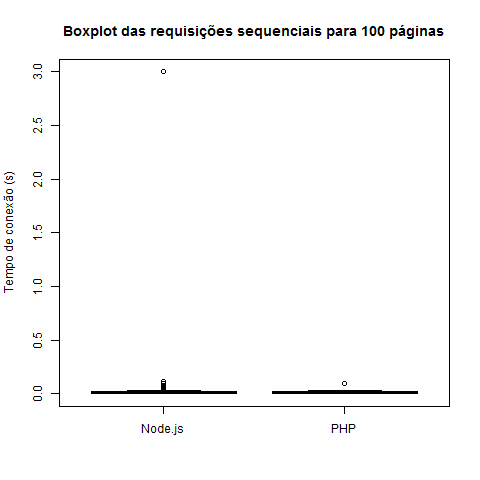
\includegraphics[scale=0.35]{plots/boxplots/sequential/CONNECT_TIME/boxplot_CONNECT_TIME_100_pages.png}
  	\caption{Boxplots de Node.js e PHP considerando tempo de conexão}
	\label{fig:boxplot_connect_time_sequential_100}
\end{figure}

\begin{figure}[h!]
\centering
  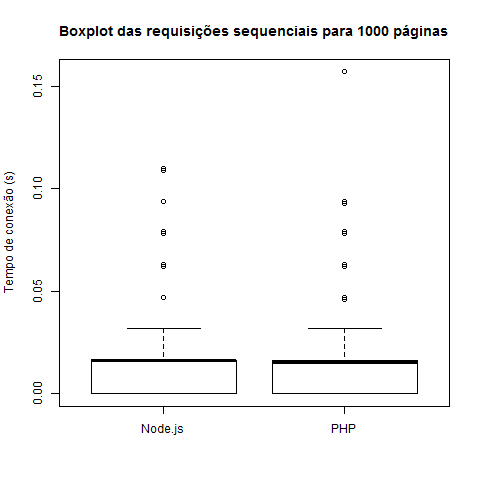
\includegraphics[scale=0.35]{plots/boxplots/sequential/CONNECT_TIME/boxplot_CONNECT_TIME_1000_pages.png}
  	\caption{Boxplots de Node.js e PHP considerando tempo de conexão}
	\label{fig:boxplot_connect_time_sequential_1000}
\end{figure}

\begin{figure}[h!]
\centering
  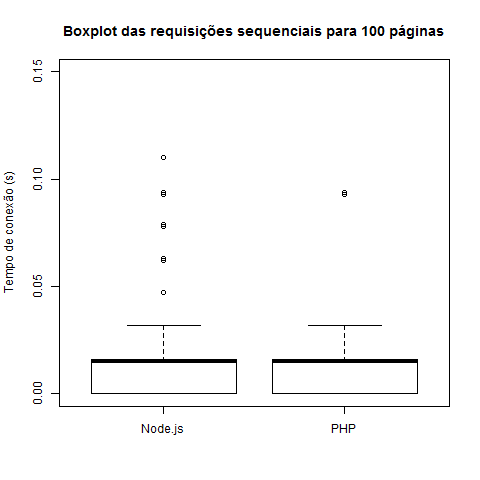
\includegraphics[scale=0.35]{plots/boxplots/sequential/CONNECT_TIME/boxplot_CONNECT_TIME_100_pages_zoom_mean.png}
  \caption{Boxplots de Node.js e PHP considerando tempo de conexão, com amplificação das médias}
  	\label{fig:boxplot_connect_time_sequential_100_zoom}
\end{figure}

A comparação anterior foi relativa às requisições quando realizadas de forma sequencial, porém ao analisar as requisições feitas de forma concorrente, o comportamento verificado foi diferente. O servidor Node.js possui uma mediana maior que o servidor PHP, considerando o envio de 100 páginas do arquivo de teste, para o tempo de conexão. O envio de um arquivo de 1000 páginas, porém, mostrou uma mudança nesse quadro, tal que o servidor Node.js obteve uma mediana de tempo de conexão mais abaixo da mediana do servidor PHP. O contraste identificado é visualizado nas figuras \ref{fig:boxplot_connect_time_concurrent_100} e \ref{fig:boxplot_connect_time_concurrent_1000}.
\\
\begin{figure}[h!]
\centering
  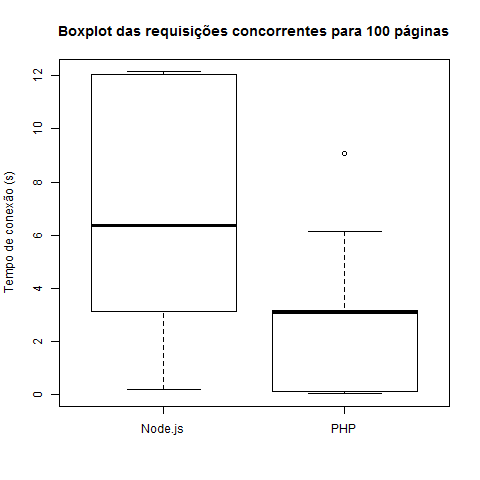
\includegraphics[scale=0.35]{plots/boxplots/concurrent/CONNECT_TIME/boxplot_CONNECT_TIME_100_pages.png}
  \caption{Boxplots de Node.js e PHP considerando tempo de conexão}
  \label{fig:boxplot_connect_time_concurrent_100}
\end{figure}

\begin{figure}[h!]
\centering
  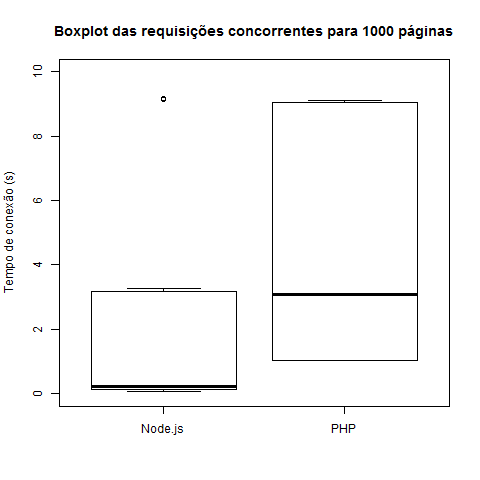
\includegraphics[scale=0.35]{plots/boxplots/concurrent/CONNECT_TIME/boxplot_CONNECT_TIME_1000_pages.png}
  \caption{Boxplots de Node.js e PHP considerando tempo de conexão}
    \label{fig:boxplot_connect_time_concurrent_1000}
\end{figure}

\subsubsection{Velocidade de transferência}
Para a variável aleatória SPEED\_DOWNLOAD, consideraremos que quanto mais alta for o seu valor, de maior performance o servidor poderá ser considerado. O que realmente faz sentido, pois indica que os usuários que requisitaram os arquivos podem ter o tempo de espera pelo arquivo reduzido. 

% Sequential

Para os valores encontrados, no primeiro cenário de teste, as medianas apresentaram-se muito próximas para os ambos os servidores. Os boxplots para este cenário, como ser visualizado na figura \ref{fig:boxplot_speed_download_sequential_100}, onde o servidor de tecnologia PHP possui mediana de 650 KB/s e enquanto Node.js aproximadamente 670 KB/s. Pode-se visualizar uma quantidade de \textit{outliers} muito grande para ambos os servidores também. Porém os dados estão mais "espalhados" quando o servidor em Node.js é utilizado. Vale ressaltar porém que a mediana das requisições em Node.js possui um valor aproximadamente o mesmo do maior valor encontrado para PHP, neste mesmo cenário de teste.

\begin{figure}[h!]
\centering
  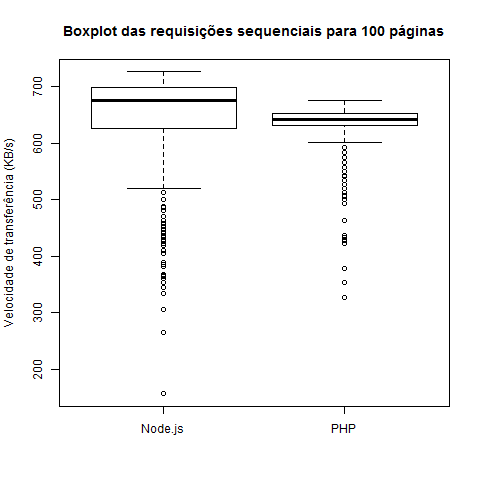
\includegraphics[scale=0.35]{plots/boxplots/sequential/SPEED_DOWNLOAD/boxplot_SPEED_DOWNLOAD_100_pages_processed.png}
  \caption{Boxplots de Node.js e PHP considerando velocidade de transferência}
    \label{fig:boxplot_speed_download_sequential_100}
\end{figure}

(Analisar o boxplot para 1000 páginas - sequential)

Um cenário um pouco diferente é percebido quando são feitas requisições para arquivos de 1000 páginas. 

\begin{figure}[h!]
\centering
  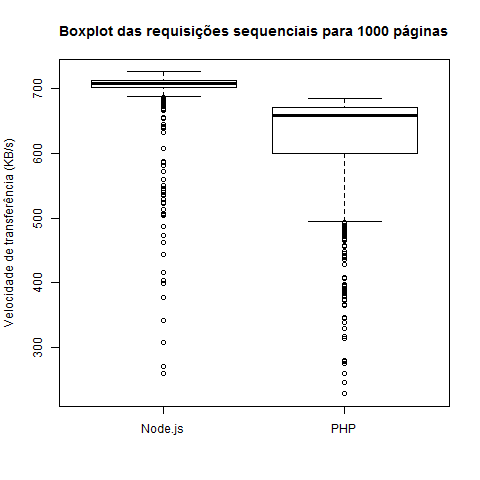
\includegraphics[scale=0.35]{plots/boxplots/sequential/SPEED_DOWNLOAD/boxplot_SPEED_DOWNLOAD_1000_pages_processed.png}
  \caption{Boxplots de Node.js e PHP considerando velocidade de transferência}
    \label{fig:boxplot_speed_download_concurrent_100}
\end{figure}

% Concurrent

Vamos considerar o cenário de teste 1, inicialmente, e podemos visualizar na figura \ref{fig:boxplot_speed_download_concurrent_100}, que a mediana de ambos os servidores é próxima, com alguns \textit{outliers} para Node.js e um quartil superior maior para o servidor PHP, indicando que temos casos que demoraram mais para realizar o \textit{download}. Um ponto interesse acontece quando aumentamos a figura \ref{fig:boxplot_speed_download_sequential_100}, para comparar as diferenças entre as medianas de uma forma mais apropriada. Essa diferença é vista na figura \ref{fig:boxplot_speed_download_concurrent_100_zoom}, nota-se uma discrepência muito maior do que vista inicialmente. Sendo a mediana de Node.js um pouco maior que 0.5 KB/s e PHP, um pouco acima 2 KB/s, sendo portanto um pouco mais rápido. 

\begin{figure}[h!]
\centering
  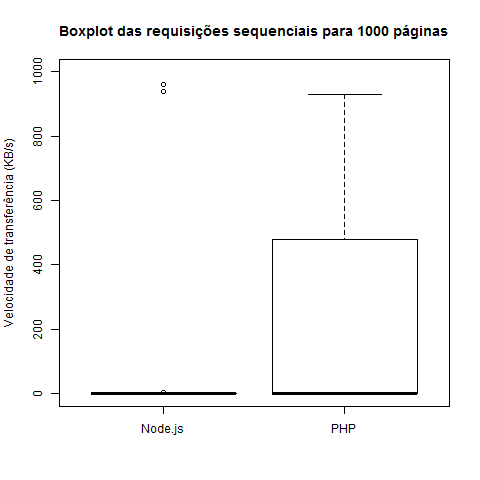
\includegraphics[scale=0.35]{plots/boxplots/concurrent/SPEED_DOWNLOAD/boxplot_SPEED_DOWNLOAD_1000_pages_processed.png}
  \caption{Boxplots de Node.js e PHP considerando velocidade de transferência}
    \label{fig:boxplot_speed_download_concurrent_100}
\end{figure}

\begin{figure}[h!]
\centering
  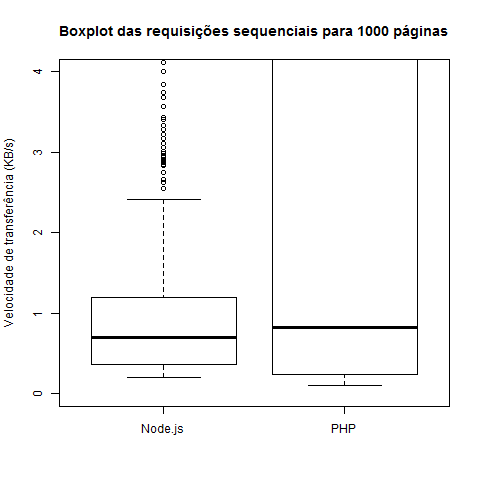
\includegraphics[scale=0.35]{plots/boxplots/concurrent/SPEED_DOWNLOAD/boxplot_SPEED_DOWNLOAD_1000_pages_processed_zoom_mean.png}
  \caption{Boxplots de Node.js e PHP considerando velocidade de transferência}
    \label{fig:boxplot_speed_download_concurrent_100_zoom}
\end{figure}

Para o segundo cenário, (...)


\subsubsection{Tempo total}
Todo

% Sequencial
% Concorrente

\subsubsection{Comparação das médias das variáveis aleatórias}
Ao comparar apenas as médias para as categorias de envio de arquivos de 100 páginas considerando sem e com concorrência.
\\
%http://tex.stackexchange.com/questions/220764/caption-of-figure-and-legend-under-the-figure
\begin{figure}

\begin{tikzpicture}
  \begin{axis}[
    xbar,
    xmax=100000.0,
    area legend,
    y axis line style = { opacity = 0 },
    axis x line       = none,
    tickwidth         = 0pt,
    enlarge y limits  = 0.3,
    enlarge x limits  = 0.02,
    symbolic y coords = {TOTAL\_TIME, SPEED\_DOWNLOAD, CONNECT\_TIME},
    nodes near coords,
    legend columns=2,
    legend cell align=left,
   	legend style={at={(0.0,0.0)},anchor=north}
  ]
  \addplot [xbar, pattern=north east lines] coordinates { 
  	(57727,TOTAL\_TIME) (5672,SPEED\_DOWNLOAD) (2193,CONNECT\_TIME) 
  };
  \addplot [xbar, pattern=dots] coordinates { 
  	(14320,TOTAL\_TIME) (1615,SPEED\_DOWNLOAD) (560,CONNECT\_TIME)
  };
  \legend{Node.js, PHP}
  \end{axis}
\end{tikzpicture}
\caption{Gráficos de médias das requisições sequenciais}
\label{fig:bar_chart_sequential}
\end{figure}

Teste para referencia \ref{fig:bar_chart_sequential}

\subsection{Testes de hipótese}
Podemos verificar pelos boxplots gerados que nenhuma das amostras coletadas possui distrubuição normal. Também foram construídos histogramas sobre os dados das amostras mas estes foram omitidos desse artigo. Notamos que a distribuição dos dados não é normal para nenhuma das amostras coletadas. Assim, iremos utilizar o teste de Wilcoxon Signed-Rank, considerando além da não-normalidade dos dados, a natureza pareada em que os dados foram coletados.

É razoável considerar que o servidor em Node.js tenha uma melhor performance em comparação a um servidor desenvolvido em PHP, principalmente pela natureza do servidor ser \textit{event-driven} para casos de entrada e saída. Para testar essa consideração, vamos utilizar as variáveis descritas anteriormente (CONNECT\_TIME, SPEED\_DOWNLOAD, TOTAL\_TIME)

É necessário identificar primeiramente a distribuição que se adeque aos conjuntos de dados. 
- Teste de aderência dos dados
- Teste de homogeneidade das variâncias
- Teste de hipóteses

\begin{hyp}[H\ref{hyp:first}] \label{hyp:first}
This is my first hypothesis.
\end{hyp}

\begin{hyp}[H\ref{hyp:second}] \label{hyp:second}
This is my second hypothesis.
\end{hyp}

\begin{center}
$H_0: \mu_X=\mu_Y$ \\
$H_1: \mu_X\neq\mu_Y$
\end{center}


\section{Conclusão}
Esse artigo apresenta um estudo comparativo entre as tecnologias Node.js e PHP para desenvolvimento de servidores \textit{web}. 
\\
Em resumo, (...)

\renewcommand\refname{Referências}

\begin{thebibliography}{4}
% \cite{paper}

\bibitem{performance_comparison}
Kai Lei, Yining Ma, Zhi Tan, \emph{Performance Comparison and Evaluation of Web Development Technologies in PHP, Python and Node.js}. \hskip 1em plus 0.5em minus 0.4em\relax IEEE 17th International Conference on Computational Science and Engineering, 2014.

\bibitem{nodejs_viable_option}
Ioannis K. Chaniotis, Kyriakos-Ioannis D. Kyriakou, Nikolaos D. Tselikas, \emph{Is Node.js a viable option for building modern web
applications? A performance evaluation study}. \hskip 1em plus 0.5em minus 0.4em\relax Springer-Verlag Wien, 2014.

\bibitem{curl_manpage}
https://curl.haxx.se/docs/manpage.html

\bibitem{node_js_oficial}
Node.js, https://nodejs.org/en/

\bibitem{php_oficial}
PHP, http://php.net/

\bibitem{lipsum}
http://www.lipsum.com/

\end{thebibliography}

\end{document}


